%%%%%%%%%%%%%%%%%%%%%%%%%%%%%%%%%%%%%%%%%%%%%%%%%%%%%%%%%%%%%%%%%%%%%%%

\chapter{Разрарботка и тестирование АПК}

%%%%%%%%%%%%%%%%%%%%%%%%%%%%%%%%%%%%%%%%%%%%%%%%%%%%%%%%%%%%%%%%%%%%%%%
В рамках командного курсового проекта по предмету "Технологии разработки ПО" во втором семестре магистратуры был разработан прототип АПК сбора климатических параметров(рис. ~\ref{fig:proto}).

\begin{figure}[H]
	\centering
	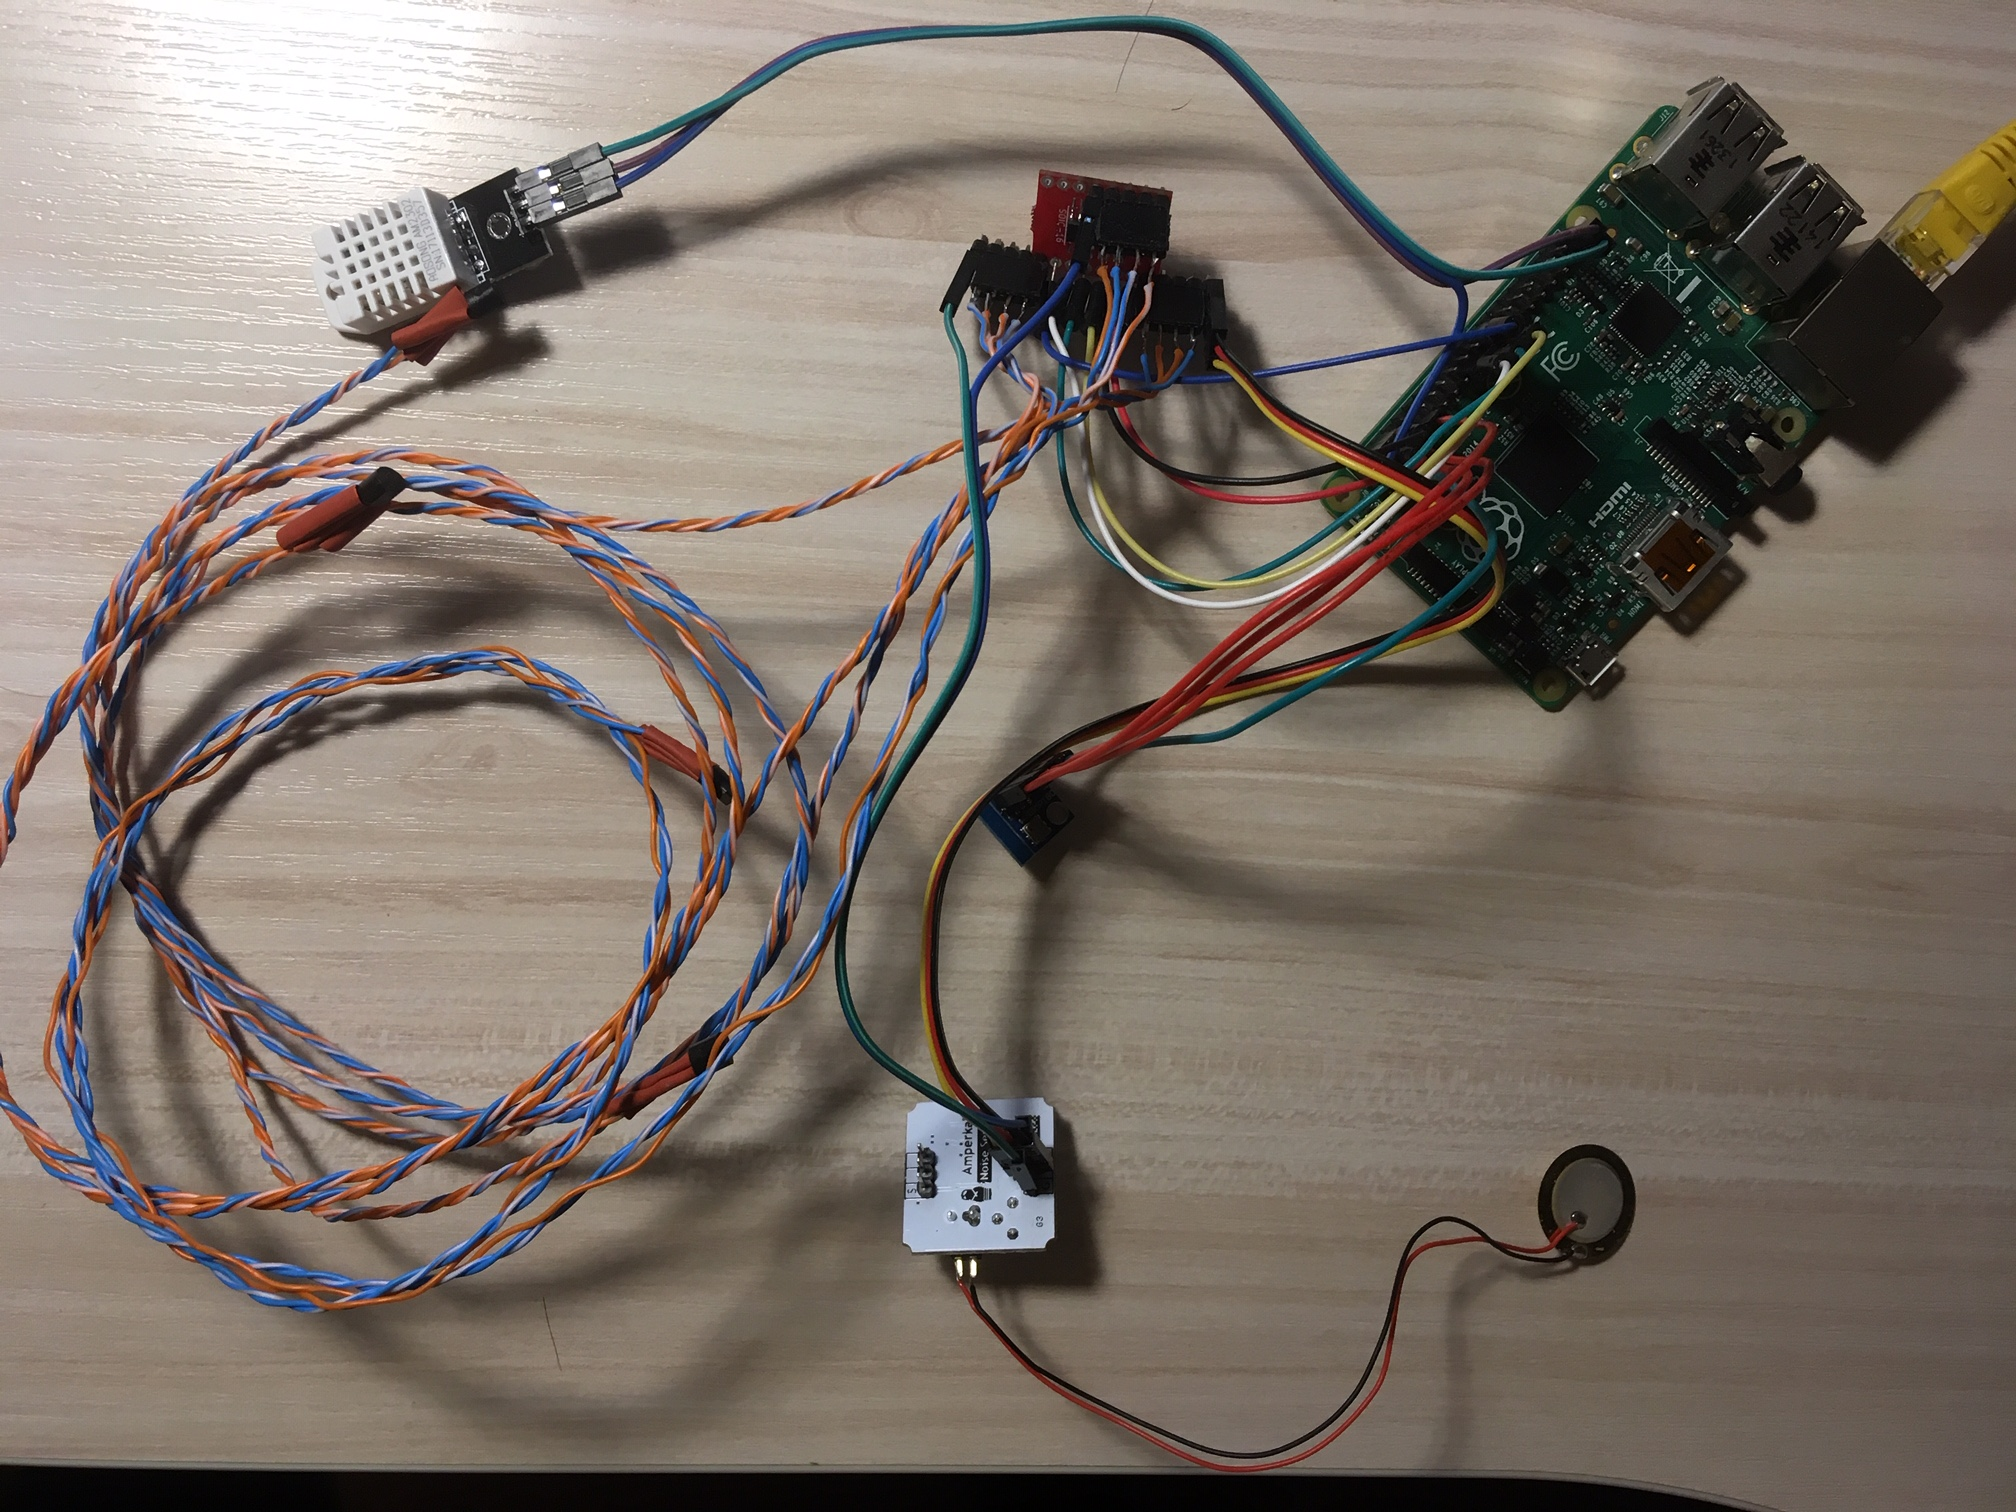
\includegraphics[width=\textwidth]{proto}
	\caption{Прототип АПК сбора климатических параметров СХД}
	\label{fig:proto}
\end{figure}
Данный прототип представляет из себя плату управления и набор датчиков, непосредственно подключенных к ней. В ходе исследовательских испытаний был выявлен ряд недостатков: 
\begin{itemize*}
	\item{Отсутствие общей платы сопряжения}
	\item{Отсутствие корпуса изделия}
	\item{Отсутствие единого блока питания}
	\item{Отсутсвие дисплея}
\end{itemize*}

Исполнение прототипа навесным монтажом обернулось постоянной проблемой отпадающих контактов, что затрудняло испытания. Кроме того, в схеме не предусмотрены подтягивающие резисторы для цифровых каналов связи, что создавало дополнительные помехи. 

Отсутствие встроенного блока питания и корпуса изделия не сказывалось на использование прототипа, однако для реального использования АПК как единицы сбора данных необходимо снабдить прототип и блоком питания и корпусом. Стоит отметить, что изменение формы и вида корпуса позволит гибко использовать прототип в различных целях.

Также, в ходе испытаний прототипа было выявлено, что при использовании прототипа в качестве системы сбора климатических параметров в стойке СХД, актуальным является отображение текущих измеряемых АПК показаний на дисплее. 

С точки зрения программного обеспечения, разработанный протоип представляет из себя набор драйверов, позволяющих обращаться к конкретному датчику и получать с него показания. Для использования прототипа как части системы сбора данных, требуется реализовать REST сервер, осуществляющий ответы на запросы текущих показаний датчиков, а также исторических показаний за период равный посленим суткам. Кроме того, для удобства отслеживания изменения параметров требуется разработать web интерфейс, отображающий текущие и исторические параметры в виде графиков.

Дополнительная аппаратная задача по добавлению дисплея для отображения текущих показаний добавляет программную задачу работы с дисплеем. 

Учитывая вышеописанные замечания, была разработана новая структура АПК сбора климатических параметров(рис. ~\ref{fig:structMSS}).
\begin{figure}[h]
	\centering
	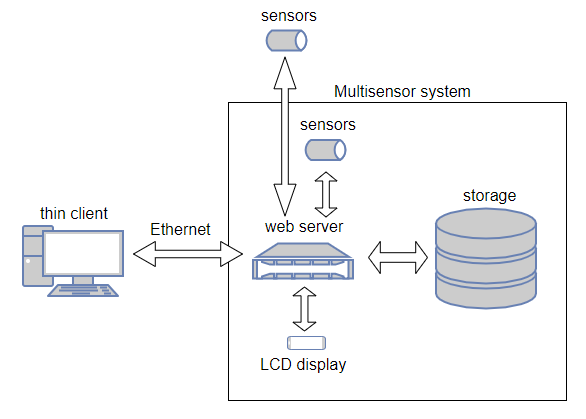
\includegraphics[width=\textwidth]{structMSS}
	\caption{Общая схема АПК}
	\label{fig:structMSS}
\end{figure}

%%%%%%%%%%%%%%%%%%%%%%%%%%%%%%%%%%%%%%%%%%%%%%%%%%%%%%%%%%%%%%%%%%%%%%%
\section{Разработка аппаратного комплекса}
%%%%%%%%%%%%%%%%%%%%%%%%%%%%%%%%%%%%%%%%%%%%%%%%%%%%%%%%%%%%%%%%%%%%%%%
Основываясь на структуре АПК, было принято решение изготовить печатную плату сопряжения датчиков и контроллера управления АПК, а также разместить на ней датчики не требующие выносного монтажа(датчик давления и датчик влажности).  
В прототипе применен 8 канальный 12 битный АЦП фирмы Microchip - mcp3208, который позволяет измерять температуру и вибрацию с достаточной точностью, при использовании аналоговых датчиков температуры, а также датчика вибрации. Для подсоединения внешних датчиков на плате выведены разъемы включающие контакты питания и сигнальные.
На рисунке  ~\ref{fig:sceme} представлена принципиальная схема платы сопряжения. 
\begin{figure}[H]
	\centering
	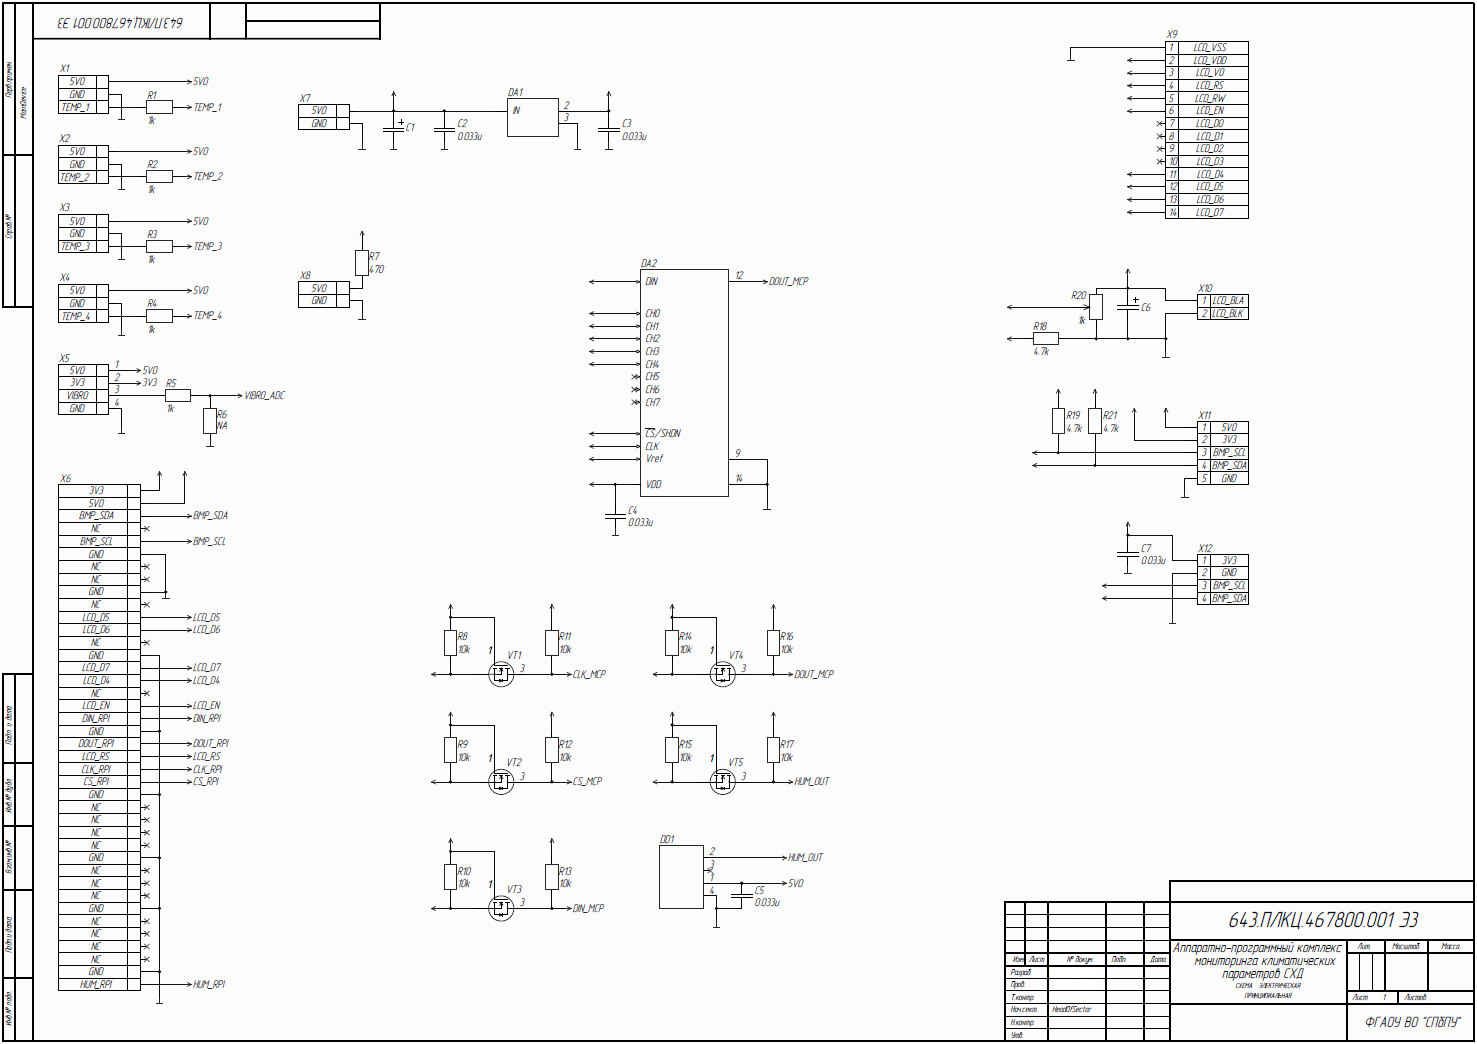
\includegraphics[angle=270,width=\textwidth]{sceme}
	\caption{Принципиальная схема платы сопряжения}
	\label{fig:sceme}
\end{figure}

Для согласования уровня напряжений управляющего устройства - 3.3в и напряжения логических сигналов АЦП - 5в была применена двунаправленная схема с MOSFET транзистором. Номиналы подтягивающих резисторов - по 10кОм. Такая схема(см. рисунок ~\ref{fig:3to5}) часто применяется в шинных системах с открытым коллектором.  Аналогично выполнено подключение датчика влажности. Кроме того были добавлены конденсаторы небольшой ёмкости для гашения дребезжаний. 
\begin{figure}[H]
	\centering
	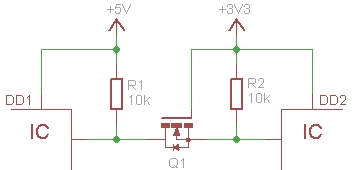
\includegraphics[width=\textwidth]{3to5}
	\caption{Схема согласования уровней напряжений на полевом транзисторе}
	\label{fig:3to5}
\end{figure}

Для вывода информации о текущих показаниях опрашиваемых датчиков был выбран символьный LCD дисплей WH1602~\cite{wh1602}. Подключение дисплея выполнено по стандартной схеме из приведенной технической документации.  

Печатная плата была разведена в CAD системе Altium Designer 18 основываясь на руководстве разработчика~\cite{altium}. 
Результат трассировки дорожек предсставлен на рисунке ~\ref{fig:board}.
\begin{figure}[H]
	\centering
	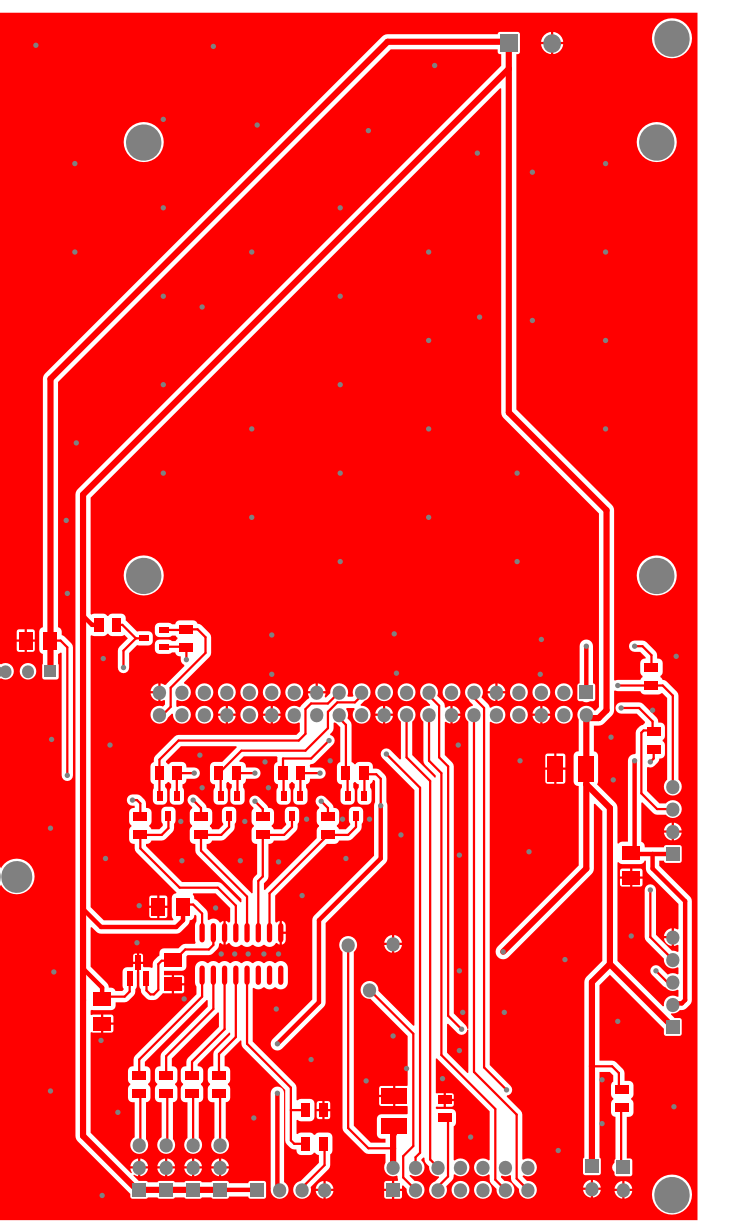
\includegraphics[angle=90,width=\textwidth]{board}
	\caption{Результат трассировки дорожек платы сопряжения}
	\label{fig:board}
\end{figure}

После разводки было заказано изготовление платы на заводе, произведен монтаж элементов.  
Изготавливаемый образец АПК предназначен для установки в серверную стойку размером 1U. Для корпусирования устройства был куплен цельный корпус стандартного размера и вырезаны необходимые отверстия для LCD дисплея, кнопки питания, светодиодной индикации и разъемов. Внутрь были смонтированы управляющее устройство, плата сопряжения и блок питания. 

Для внешних датчиков и иных подключений(Ethernet, питание) были установлены разъемы в корпус изделия. Для уменьшения шумов в аналоговых датчиках провода были заменены на экранированные. 
Внешний вид изготовленного прототипа АПК представлен на ~\ref{fig:result}.

\begin{figure}[h]
	\centering
	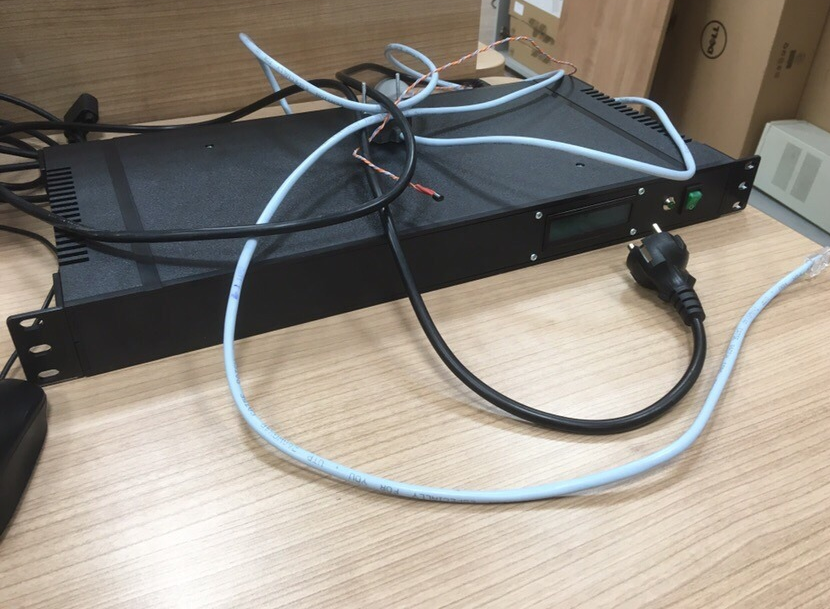
\includegraphics[width=\textwidth]{result}
	\caption{Внешний вид изготовленного АПК сбора климатических параметров}
	\label{fig:result}
\end{figure} 

Выведение контактов интерфейса I2C и питания(3.3в и 5в) на разъем в корпусе устройства позволяет использовать данный разъем для подключения дополнительного датчика с данным интерфейсом, что придает системе гибкость. Также, на корпус устройства выведены разъемы аналоговых датчиков температуры (подсоединение на соответствующие каналы АЦП), что позволяет заменить датчики температуры на иные аналоговые без изменений в схеме подключения. Замена внутренних датчиков(влажнсти и давления) не предусмотрена - датчики будут присутствовать в любом исполнении АПК. 


%%%%%%%%%%%%%%%%%%%%%%%%%%%%%%%%%%%%%%%%%%%%%%%%%%%%%%%%%%%%%%%%%%%%%%%
\section{Разработка программного комплекса}
%%%%%%%%%%%%%%%%%%%%%%%%%%%%%%%%%%%%%%%%%%%%%%%%%%%%%%%%%%%%%%%%%%%%%%%
Придерживаясь ранее разработанной структуры(рис. ~\ref{fig:structMSS}), рассмотрим подробнее программную часть АПК. 
Основной частью программного обеспечения является сервер, написанный на Python с использованием библиотеки http.server. При обработке одного из запросов происходит вызов функций драйверов датчиков или же чтение исторических данных из хранилища.
При старте программы происходит старт сервера и параллельный запуск в разных потоках функции отображения информации на LCD дисплей и записи данных в хранилище. 

Для осуществелния обмена информацией с LCD  дисплеем была использована библиотека Adafruit\_CharLCD. Перед началом работы с дисплеем производится его инициализация(указываются порты подключения, размерность и наличие подсветки). Функция вывода на экран информации осуществляет в бесконечном цикле формирование строк вывода из текущих показаний и чередование выводимых датчиков с задержкой в 5 секунд. 

Для хранения данных был выбран наиболее простой вариант - показания каждого из датчиков хранятся в отдельном файле. Функция записи данных циклически осуществляет опрос датчиков и дозапись показаний. Реализована ротация файла на 100 показаниях. Период опроса сенсоров составляет 900с, что соответствует хранению истории чуть больше чем за прошедшие сутки. 

Для предотвращения ошибок доступа к общей памяти разных потоков, использовалась блокировка ресурса.

Разработанное программное обеспечение представляет из себя SystemD сервис~\cite{SystemD}, запускающийся при старте ОС управляющего устройства. При старте сервис поднимает сервер, написанный на Python, выполняющий сбор данных с датчиков и сохранение показаний в хранилище. Чтение текущих показаний с датчиков возможно с помощью клиента (браузера или самописного) с использованием определенного REST API. Графическое отображение текущей и исторической информации осуществляется с помощью веб-клиента. 

\begin{figure}[h]
	\centering
	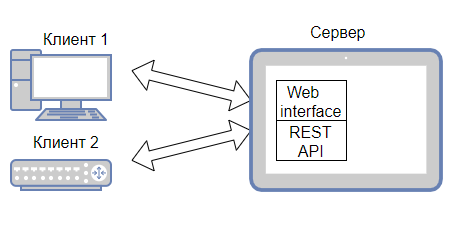
\includegraphics[width=3.0in]{cliserv}
	\caption{Клиент-серверная архитектура}
	\label{fig:cliserv}
\end{figure}

Для разработанной системы сбора и отображения климатических параметров СХД был написан веб-интерфейс, визуализирующий текущие показания датчиков климатических параметров и исторические показания, накопленные за последние 100 измерений (24 часа). 

Веб-интерфейс написан с использованием фреймворка JQuery ~\cite{jQuery}. Для построения графиков использовалась общедоступная библиотека Chart.js~\cite{Chartjs}. С помощью ajax запросов реализуется опрос сервера: 
\begin{itemize*}
	\item{Каждые 10с запрос текущих показаний датчиков (срез по всем датчикам)}
	\item{Каждые 100с запрос исторических показаний каждого из датчиков}
\end{itemize*}

Первоначальная иницализация представляет из себя последоваельный вызов функий initDynamicCharts(), pollSensors() и pollSensorsArray(). Функция initDynamicCharts() устанавливает цвета для графиков отображающих динамику текущих показаний датчиков.  Функция pollSensors() отправляет get запрос на чтение текущих показаний, парсит пришедший json и вызывает функции обновления updaeChart() для каждого из графиков. 
Функция pollSensorsArray() отвечает за обновление исторических данных, в теле функции для каждого исторического графика вызывается функция pollSensor(). 

Функция pollSensor() отправляет соответствующий входным аргументам get запрос и производит подсчет метрик среднего, минимального и максимального значений с последующим обновлением.

Обновление показаний производится циклически с интервалами 10с и 100с для текущих данных и исторических соответственно с помощью функции window.setInterval(). 

Соответствующий листинг приведен в приложении...................
\begin{figure}[h]
	\centering
	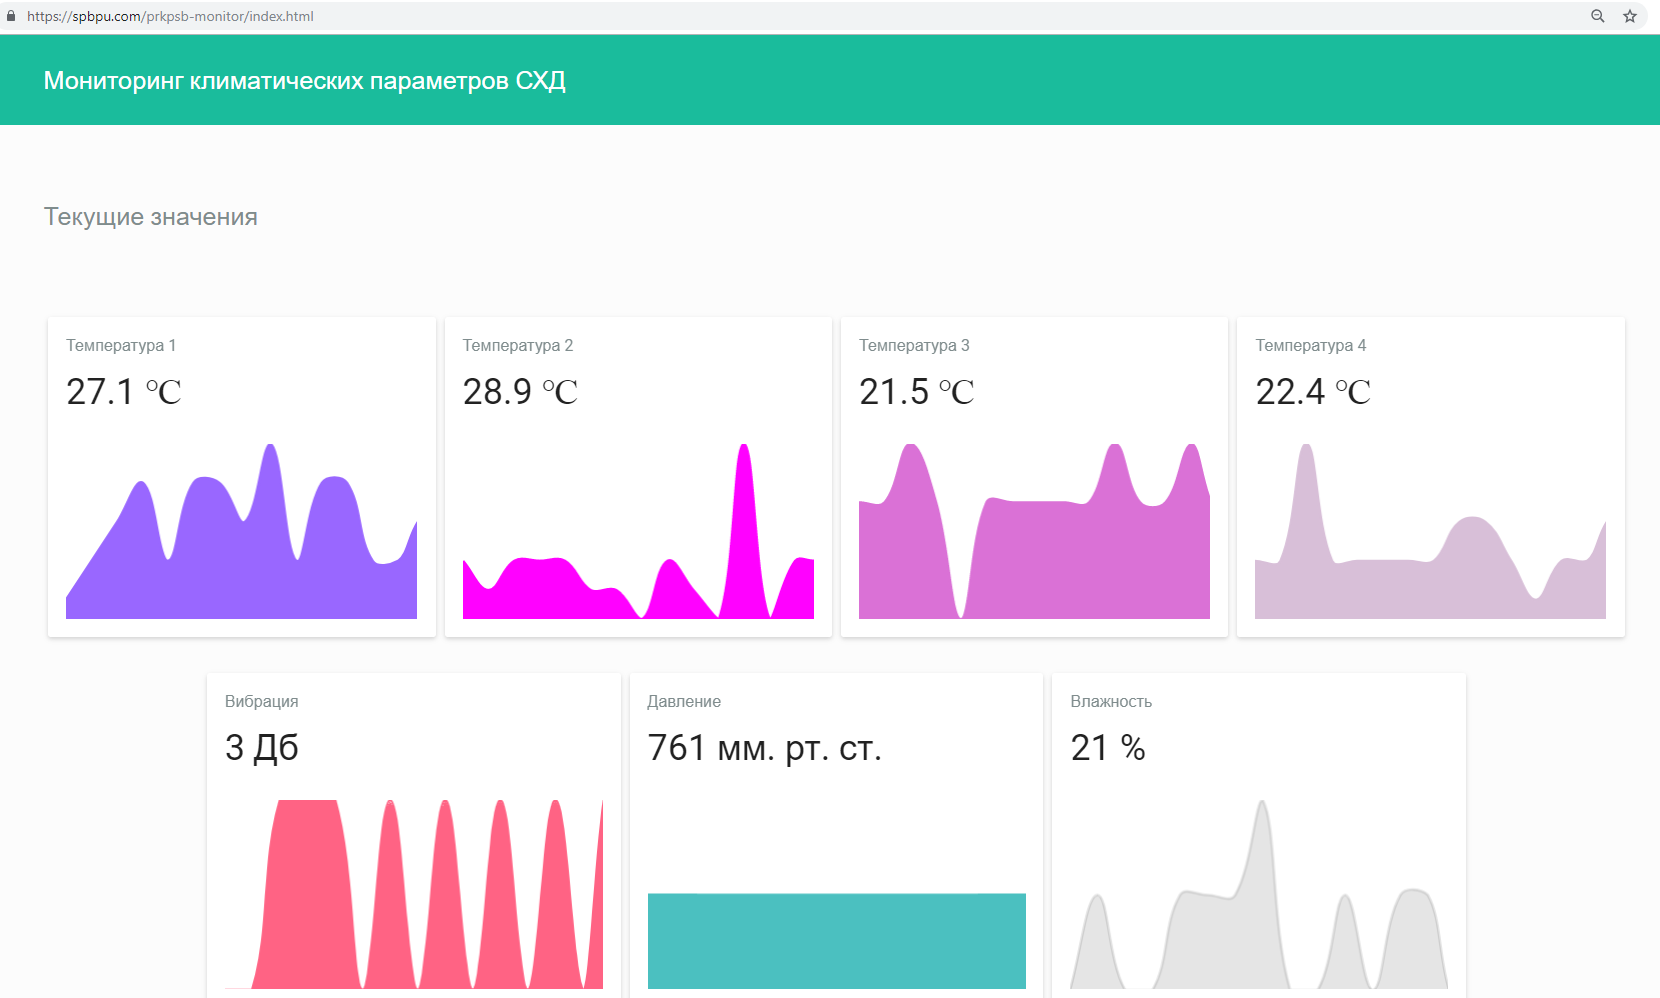
\includegraphics[width=\textwidth]{web}
	\caption{Внешний вид веб-интерфейса(текущие показания)}
	\label{fig:web}
\end{figure}

Внешний вид веб-интерфейса представлен на рисунках ~\ref{fig:web} -~\ref{fig:web2}.

\begin{figure}[h]
	\centering
	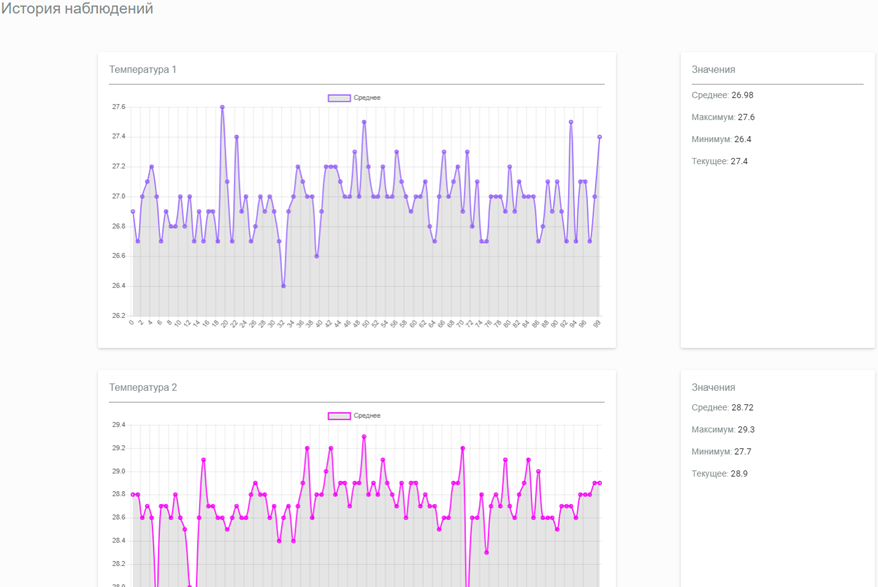
\includegraphics[width=\textwidth]{web2} 
	\caption{Внешний вид веб-интерфейса(исторические показания)}
	\label{fig:web2}
\end{figure}

Для проверки работоспособности комплекса....



%%You can use all kinds of abbreviations that don't mean anything, but add
%%a false sense of importance and significance to your work. Some of these
%%abbreviations are:
%
%%\begin{itemize*}
%%\item eXtensible Markup Language~(XML)
%%\item JavaScript Object Notation~(JSON)
%%\item Yet Another Markup Language~(YAML)
%%\end{itemize*}
%


%%\begin{table}
%%\captionsetup{skip=5pt}
%%\caption{Решетка замечательности аббревиатур}
%%\centering
%%XML < JSON < YAML
%%\end{table}


%%%%%%%%%%%%%%%%%%%%%%%%%%%%%%%%%%%%%%%%%%%%%%%%%%%%%%%%%%%%%%%%%%%%%%%%%%%%%%%%
%%\section{}
%%%%%%%%%%%%%%%%%%%%%%%%%%%%%%%%%%%%%%%%%%%%%%%%%%%%%%%%%%%%%%%%%%%%%%%%%%%%%%%%

